\section{Abalone Scatter Plot}

\begin{figure}[H]
  \centering
  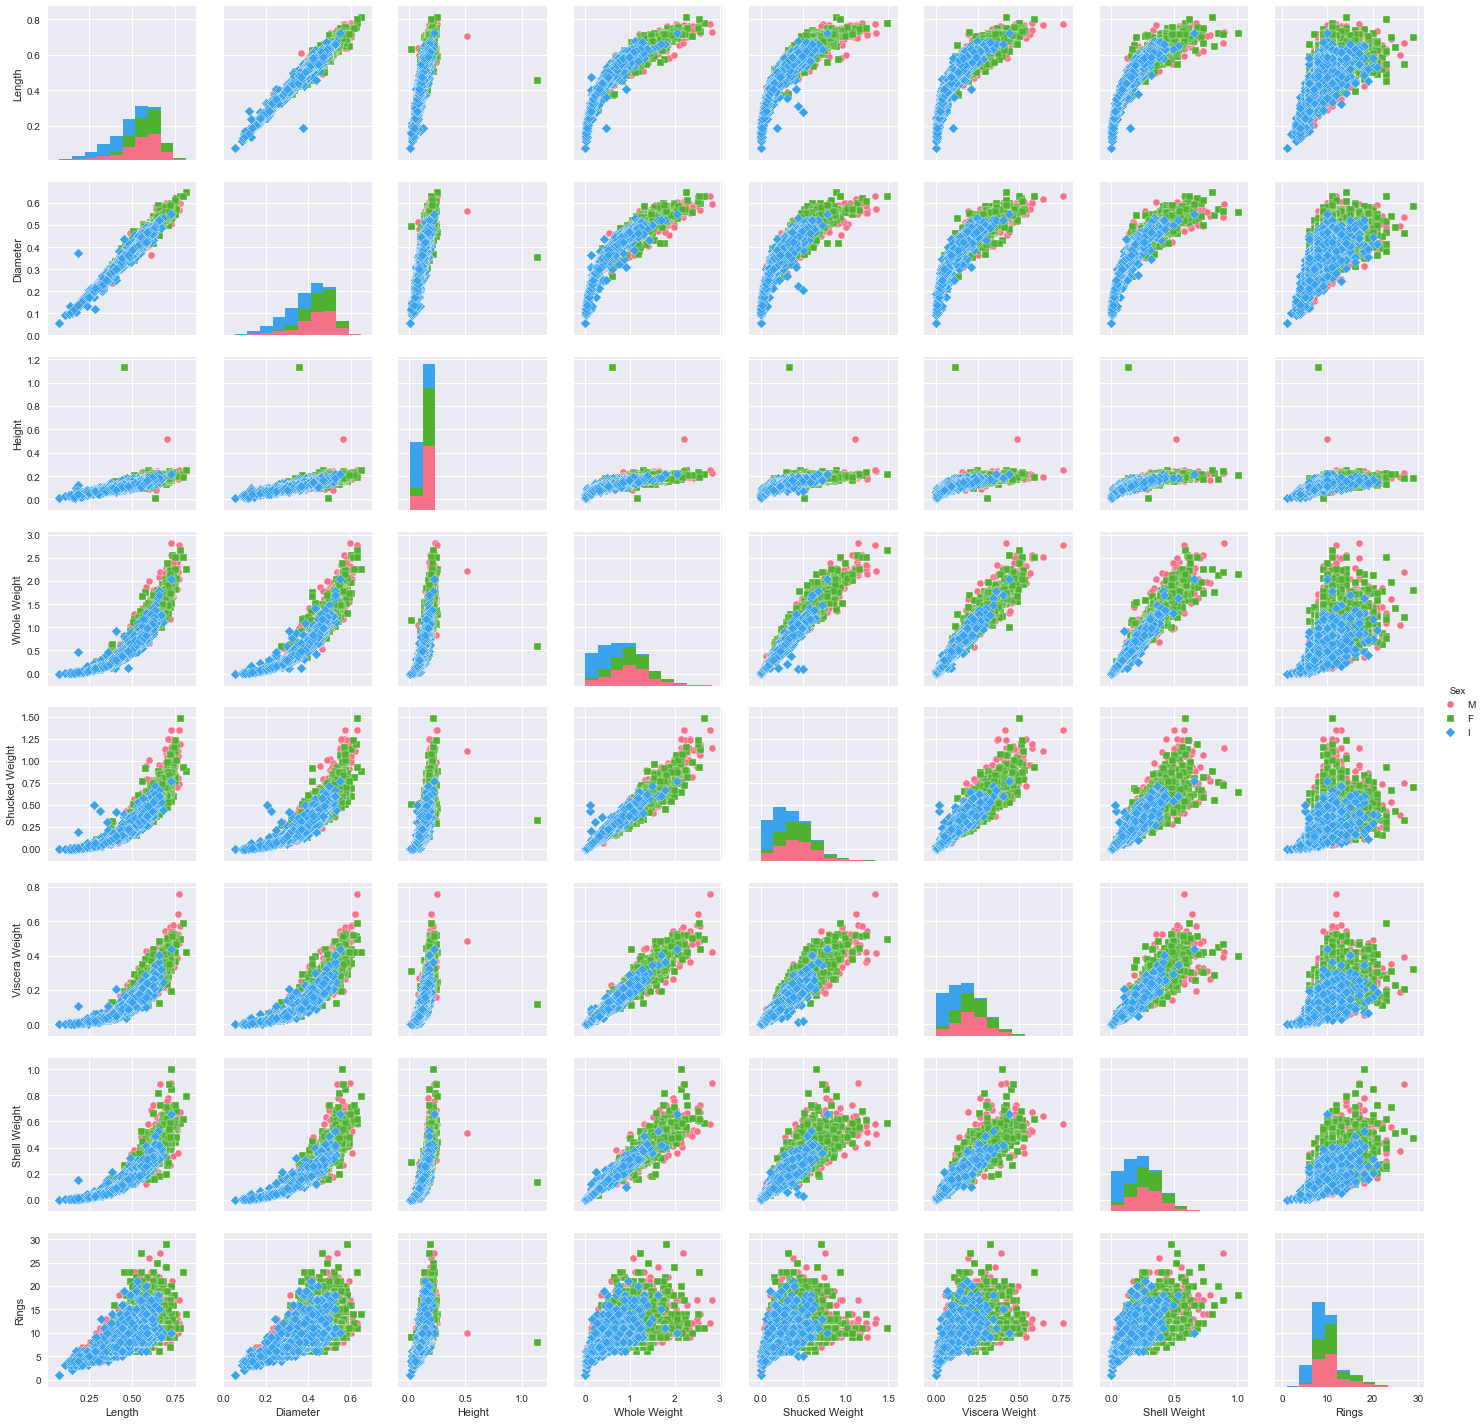
\includegraphics[scale=0.5,width=100mm]{./images/abalone-scatter-plot.png}
  \caption{Scatter Plot of the abalone dataset}
  \label{fig:abalones-scatter-plot}
\end{figure}

Figure \ref{fig:abalones-scatter-plot} shows a scatter plot of the entire dataset. It is immediately clear that there is a high degree of correlation. For example, length and diameter seem very correlated. Figure \ref{fig:abalones-scatter-plot} may be a little hard to read as there is a lot of data. Figure \ref{fig:abalones-scatter-plot-condensed} shows a more condensed version with the most highly correlated features.

\begin{figure}[H]
  \centering
  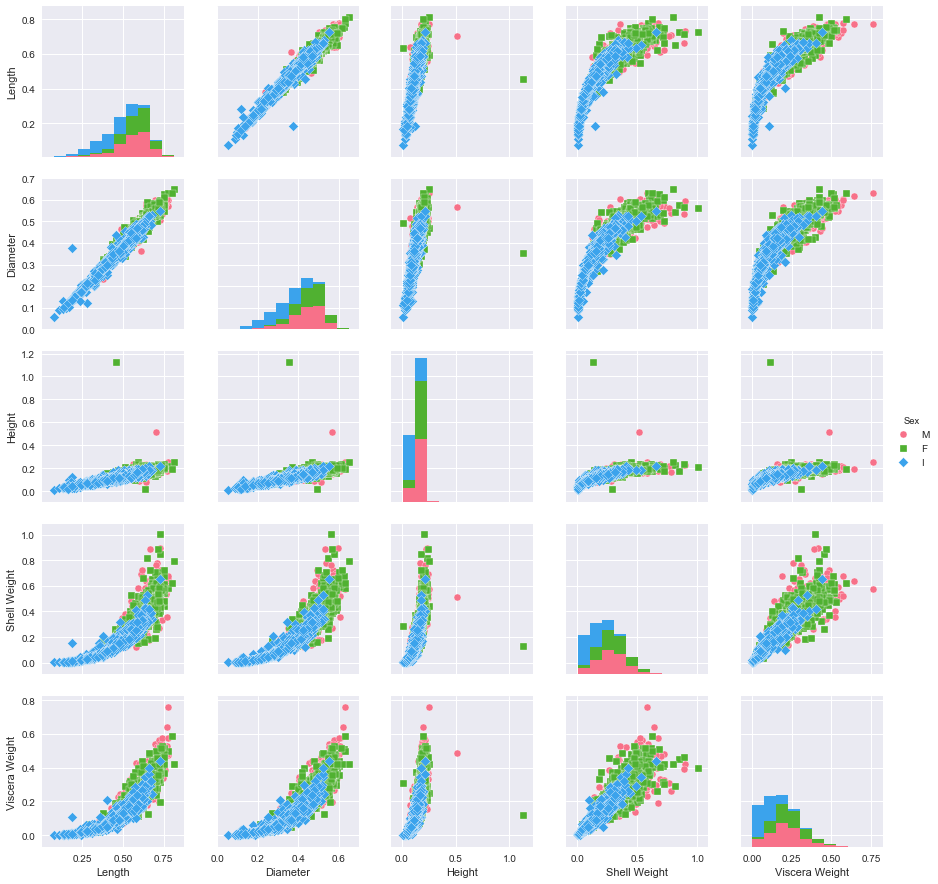
\includegraphics[scale=0.5,width=100mm]{./images/abalone-scatter-plot-condensed.png}
  \caption{Scatter Plot of the abalone dataset}
  \label{fig:abalones-scatter-plot-condensed}
\end{figure}

\begin{figure}[H]
  \centering
  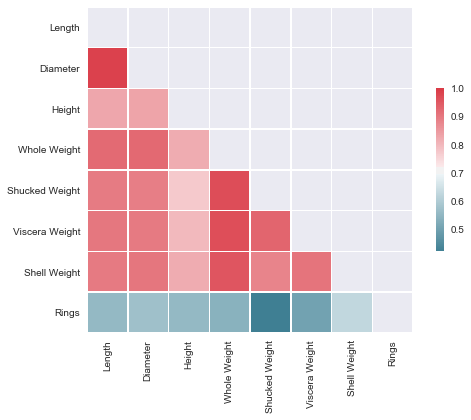
\includegraphics[scale=0.5,width=100mm]{./images/abalone-heatmap.png}
  \caption{Heat-map showing most highly correlated features}
  \label{fig:abalones-heatmap}
\end{figure}

Figure \ref{fig:abalones-heatmap} shows a heat-map displaying the most correlated features. Length, height, and diameter seem to be the most highly correlated. This is interesting because using physics we could turn these 3 features into one in the form of a volume feature. Whole weight, shucked weight, viscera weight and shell weight again all seem highly correlated. This is a bit confusing as one would expect some degree of difference between the sexes infant, male and female. Perhaps there is not that much of a difference between the sexes. Interestingly rings itself does not seem to be correlated much to any feature. This makes me question how well our regression model will work. 

As mentioned above at this stage I made the decision to create a new feature called volume. This would equal the result of the formula below.

\begin{equation}
    volume = length \times diameter \times height
\end{equation}